\documentclass[conference]{IEEEtran}
\usepackage{todonotes}
\IEEEoverridecommandlockouts
% The preceding line is only needed to identify funding in the first footnote. If that is unneeded, please comment it out.
\usepackage{cite}
\usepackage{amsmath,amssymb,amsfonts}
\usepackage{algorithmic}
\usepackage{graphicx}
\usepackage{textcomp}
\usepackage[utf8]{inputenc}
\usepackage{hyperref}
\usepackage{amsthm, amssymb,amsmath}
\usepackage{mathrsfs}
\usepackage{mathtools}
\usepackage{pgfplots}
\usepackage{todonotes}
\usepackage{dsfont}
\usepackage{enumitem}
\usepackage[capitalise,nameinlink]{cleveref}
\usetikzlibrary{shapes}

\renewcommand{\:}{\mathrel{\coloneqq}}
\renewcommand{\=}{\ensuremath{\eqqcolon}}
\renewcommand{\epsilon}{\varepsilon}
\usepackage[caption=false, font=normalsize, labelfont=sf, textfont=sf]{subfig}
\newcommand{\dd}{\ensuremath{\,\mathrm{d}}}
\newcommand{\ddt}{\ensuremath{\tfrac{\dd}{\dd t}}}

\newcommand{\R}{\ensuremath{\mathbb{R}}}
\newcommand{\N}{\ensuremath{\mathbb{N}}}

\newcommand{\rr}{\text{r}}
\newcommand{\nr}{\text{nr}}

\date{\today}
\newtheorem{Definition}{Definition}
\newtheorem{Routing}{Routing}
\newtheorem{Results}{Results}
\newtheorem{Lemma}{Lemma}
\newtheorem{Corollary}{Corollary}
\newtheorem{Assumption}{Assumption}

\newtheorem{Remark}{Remark}
\newtheorem{Example}{Example}
\newtheorem{Theorem}{Theorem}
\newtheorem{Challenge}{Challenge}
\newtheorem{Proposition}{Proposition}

\newcommand{\0}{\ensuremath{\boldsymbol{0}}}
\newcommand{\A}{\mathcal{A}}
\newcommand{\V}{\mathcal{V}}
\newcommand{\C}{\mathcal{C}}
\newcommand{\cS}{\mathcal{S}}
\newcommand{\T}{\mathcal{T}}

\newcommand{\fR}{\mathfrak{R}}
\newcommand{\fRD}{\mathfrak{RD}}
\newcommand{\fRL}{\mathfrak{RL}}
\newcommand{\fRU}{\mathfrak{RU}}


\newcommand{\source}{\mathcal O}
\newcommand{\sink}{\mathcal D}
\newcommand{\OD}{\source\sink}
\newcommand{\Aout}{\mathcal{A}_{\textnormal{out}}}
\newcommand{\Ain}{\mathcal{A}_{\textnormal{in}}}
\newcommand{\vout}{v_{\text{tail}}}
\newcommand{\vin}{v_{\text{head}}}
\newcommand{\paths}{\mathcal{P}}
\newcommand{\bx}{\boldsymbol{x}}
\newcommand{\bg}{\boldsymbol{g}}
\newcommand{\bu}{\boldsymbol{u}}
\newcommand{\btau}{\boldsymbol{\tau}}
\newcommand{\btheta}{\boldsymbol{\theta}}
\newcommand{\bb}{\boldsymbol{b}}
\newcommand{\bh}{\boldsymbol{h}}
\newcommand{\bk}{\boldsymbol{k}}
\newcommand{\bm}{\boldsymbol{m}}
\newcommand{\bp}{\boldsymbol{p}}
\newcommand{\bs}{\boldsymbol{s}}
\newcommand{\bX}{\boldsymbol{X}}
\newcommand{\app}{\text{r}}
\newcommand{\napp}{\text{nr}}
\newcommand{\shortp}{\mathcal{Y}}
\newcommand{\ord}{\boldsymbol{\text{Ord}}}
\newcommand{\e}{\mathrm{e}}
\DeclareMathOperator*{\argmin}{arg\,\min}
\newcommand{\ext}{\textbf{\textnormal{ext}}}


\newcommand{\Id}{\mathrm{Id}}
\newcommand{\bcX}{\boldsymbol{\mathcal{X}}}
\newcommand{\Int}{\ensuremath{\int\limits}}

\newcommand{\len}{\textnormal{len}}
\newcommand{\todoAll}[1]{\todo[inline,color=red!30!yellow]{All: #1}}

\newcommand{\xslnote}[1]{{\bf\color{red}(#1 -- Sherry)}}

\newcommand{\ggnote}[1]{{\color{blue}(#1)}}
\newcommand{\XXX}{{\color{magenta}XXX}}



\begin{document}

\title{A unified software framework for solving traffic assignment\\
%{\footnotesize \textsuperscript}
\thanks{This work is supported in part by the Office of Science of the
 U.S.~Department of Energy under contract No.~DE-AC02-05CH11231.}
}

\author{\IEEEauthorblockN{ Juliette Ugirumurera}
\IEEEauthorblockA{\textit{Computational Research Division} \\
\textit{Lawrence Berkeley National Laboratory}\\
Berkeley, California \\
ugirumurera@lbl.gov}
\and
\IEEEauthorblockN{Gabriel Gomes}
\IEEEauthorblockA{\textit{Partners for Advanced Transportation Technology} \\
\textit{University of California Berkeley}\\
Berkeley, California \\
gomes@path.berkeley.edu}
\and
\IEEEauthorblockN{Emily Porter}
\IEEEauthorblockA{\textit{Department of Civil and Environmental Engineering} \\
\textit{University of California Berkeley}\\
Berkeley, California \\
emily.porter@berkeley.edu}
\and
\IEEEauthorblockN{Xiaoye S. Li }
\IEEEauthorblockA{\textit{Computational Research Division} \\
\textit{Lawrence Berkeley National Laborator}\\
Berkeley, California \\
 xsli@lbl.gov}
\and
\IEEEauthorblockN{Alexandre Bayen}
\IEEEauthorblockA{\textit{Department of Electrical Engineering and Computer Science} \\
\textit{University of California Berkeley}\\
Berkeley, California \\
bayen@berkeley.edu}
}

\maketitle


\begin{abstract}
This paper presented a general variational inequality formulation that unify static and dynamic traffic assignment problems. From this formulation, we developed a modular and extendable software framework. The framework does not impose a traffic model, unlike existing dynamic traffic assignment software tools, which tend to favor simulation-based traffic models. Rather our software framework serves as platform to try different static and dynamic models and traffic assignment solution algorithms. It currently supports three different traffic models: a static model, a cell-based model, and the Marchant-Nemhauser model. It also includes the Frank-Wolfe algorithm, the Extra Projection method and the method of successive averages to solve the traffic assignment problems. The perfomance of the software is demonstrated with numerical results. 
\end{abstract}

\begin{IEEEkeywords}
\end{IEEEkeywords}

\section{Introduction}
\label{sec:intro}
\todo[inline]{I don't think the terms traffic assignment and route choice are used interchangeably}
The term \textit{traffic assignment} (or route choice, or route assignment) captures a large array of problems concerning the distribution of traffic over a network. Traffic assignment problems arise in transportation planning applications, such as in the traditional ``four-step'' procedure, where it occupies the final step, following trip generation, trip distribution, and mode choice \cite{mcnally2007four}.  The fundamental principle that guides most traffic assignment models is Wardrop's principle \cite{wardrop1952some}, which states that amongst the available alternatives, drivers will select routes that minimize their travel times. Because the speed of traffic tends to decrease as the number of vehicles on the route increases, Wardrop's principle leads to an iterated game in which drivers test new routes, day after day, until they converge to a Nash equilibrium, a.k.a. a \textit{user equilibrium}. The term is also used for problems that involve a single decision maker, who prescribes the routes for users in order to optimize some system-level performance metric, e.g. total travel time, emissions, energy consumption. These are mathematical programs, and their solutions are known as \textit{system optimal} assignments. We will focus in this paper on user equilibrium traffic assignments. \todo[inline]{might be nice to specify Wardrop's 1st and 2nd principles}

Since the pioneering work of Wardrop, the mathematical and numerical study of traffic assignment has progressed at a moderate pace. \todo[inline]{"moderate pace" seems weird. like as opposed to fast? what is fast? what is slow?} This is perhaps mostly due to a historical scarcity of traffic data and network information, but also because of the difficulty of the problem. [CCC] gives several examples in which problems could not be solved for networks of useful size. It is not surprising therefore that the problem has received renewed interest with recent increases in traffic and network data, and computational power. Also driving this renewal are concerns about the `unintended consequences' of the widespread use of routing apps \cite{traffic_apps}, as well as advances in autonomous driving technologies.

An investigation into the techniques of traffic assignment reveals a multitude of models, numerical methods, and performance metrics. \todo[inline]{when we say "models" we are referring to models of traffic flow dynamics - is it clear to just say "models"?} As is usually the case, the more detailed the model, the more expensive the computation. However it is not clear under which circumstances the additional effort (or investment in computational resources) is necessary. For example, although it is usually agreed that dynamical models that capture the essential phenomenon of congestion are desirable, it is also true that the computation (as well as network configuration effort) involved in solving dynamic traffic assignment (DTA) problems can be large. On the other hand, existing static planning methods cannot fully model traffic congestion because of their inability to represent queue formation and dissipation when traffic demand exceeds road capacities\cite{nie2010solving}. 

This paper presents a software framework for addressing such questions. The software is based on the formulation of traffic assignment as a \textit{variational inequality}, introduced by Nagurney \cite{nagurney2013network}. This is a very general formulation, as it requires only continuity (\XXX TRUE?) of the traffic model. Hence, it covers a wide range of models: static and dynamic, macroscopic and microscopic, `analytical' and `simulation-based', etc. The software is modular and extensible, in the sense that it provides interfaces for incorporating new models, cost functions, and numerical solvers. 

There are many other programs, both commercial and shared, that solve dynamic traffic assignment problems. 

\ggnote{I want to de-emphasize the analytical vs simulation-based dichotomy because I don't understand it. Is beats analytical or simulation-based. If simulation-based, then CTM is simulation-based? Most people would disagree, because the line is very fuzzy, and really the distinction makes little sense (as our framework demonstrates). Instead lets focus on modularity: All others (I hope) bake in the model, cost function, and solver.}

\ggnote{The list needs to be fleshed out a bit. For each, can we answer these questions: what is the problem being solved? What is the model? What is the solver algorithm? Then we can categorize them in some way.}

\begin{itemize}
\item DTALite \cite{zhou2014dtalite} is a DTA software package with a queue-based traffic simulator. DTALite uses agent-based algorithm to calculate dynamic traffic equilibrium.
\item Dynameq \cite{mahut2010traffic} software provides a vehicle-based traffic simulation with capacity to determine dynamic user equilibrium.  
\item DynaMIT-P \cite{DynaMIT,ben2001dynamit} is simulation-based DTA system designed to evaluate transportation
systems at the planning level. It comprises a demand and a supply simulator that communicate to produce a user equilibrium routing guidance using the rolling horizon process. 
\item DYNASMART-P \cite{DYNASMART,mahmassani2004dynasmart} is a simulation-based DTA tool based on the the mesoscopic traffic simulator DYNASMART. 
\item DynusT \cite{chiu2011dynust} is a simulation-based DTA software that use a gap function vehicle-based solution algorithm to determine user equilibrium.
\item INTEGRATION \cite{rakha2012integration} is DTA tool that uses a trip-based microscopic traffic model. It includes several methods to calculate DTA user equilibrium. 

\end{itemize}

In contrast to these, the software described here does not prescribe the model, cost-function, or numerical method, but rather serves as a test platform for comparing different options, both in terms of computation and the solutions they produce. The code can be found here \cite{ta_solver}.


%%%%%%%%%%%%%%%%%%%%%%%%%%%%%%%%%%%%%%%%%%%%%%%%%%%

% In addition, VI's extension and sensitivity analysis can be conveniently performed \cite{peeta2001foundations}. 
% [GG: This sounds like it might be important, but I am not sure what it is, or if it compares favorably to other sensitivity analyses, eg lagrange multipliers in optimization problems]

% Though the theory of DTA is still relatively undeveloped, variational inequality (VI) has proven to provide a unified formulation to address various classes of equilibrium and equivalent optimization problems in the DTA context. 
% [GG: I incorporated this idea in the text]
 
%Static methods were developed for long term transportation planning and are not applicable in dynamic route guidance systems that require the ability to solve transportation problems in real time\cite{boyce1989route}. 
% [GG: This is too strong of an assertion for my taste]

% In recent years, dynamic traffic assignment (DTA) has gained heightened interest, as researchers and practitioners are recognizing the need to predict the spatio-temporal evolution of traffic and the limitations of  static traffic assignment methods\cite{peeta2001foundations}. 
% [GG: The reference here is too old to be recent. Is there something more recent?]

% In this paper, we extend VI formulation to unify analytical DTA models with simulation-based DTA models. 
% [GG: I dont want to say that we did it, because most people wouldnt consider CTM a simulation. I'd rather say that we created a framework that will support it.]

% Simulation-based DTA methods compliment analytical techniques by addressing the shortcomings of analytical link models and exit functions in reproducing dynamic traffic interactions, satisfying First-In-Fist-Out property, and replicating complex vehicles and multi-user class interactions. 
% [GG: The line between "analytical" and "simulation-based" is artificial. I think we should move beyond and speak at a higher level than that false debate. I dont understand the difference between "analytical" and "simulation-based" anyway.]

% VI formulations can model more realistic traffic scenario by bypassing the issues of solution intractability associated with other analytical DTA methods such as mathematical programming and optimal control formulations. 
% [GG: This is not true.]


% our software is the first to combine simulation-based DTA models with analytical methods including mathematical programming and optimal control into one software platform. In addition, our software framework is based on a clear underlying VI DTA formulation. The general VI formulation determines the overall software architecture, but also provide a way to incorporate any type of DTA problem that can be represented with VI. 
% [GG : I really would rather not make grand claims. The clarity we've gained is only relative to my ignorance when we started. But there are people for whom everything we say here is obvious.]

\section{Problem formulation}
\label{sec:formulation}
The goal of the problem is to find a demand assignment that produces an equilibrium state trajectory in the sense of Wardrop\cite{wardrop1952some}. The traffic network  is represented as a graph. Vehicles enter and exit the network through origin and destination nodes. They travel through the network following \textit{paths}. 

\vspace{1em}

\begin{tabular}{ll}
$w\in\mathcal{W}$ & all origin-destination (OD) pairs. \\ 
$d_w : [0,T]\rightarrow \mathbb{R}^+ $  & Demand for OD pair $w\in\mathcal{W}$. \\ 
$\mathcal{P}_w$ & Set of available paths for $w\in\mathcal{W}$. \\
$\mathcal{P}=\{ \mathcal{P}_w \}_{w\in \mathcal{W}}$ & All paths. \\ 
$h_p : [0,T]\rightarrow \mathbb{R}^+ $ & Demand on path $p$. \\
$h=\{h_p | p\in\mathcal{P}\}$ : & Demand assignment.
\end{tabular}

\vspace{1em}

The demand $d_w$ for an OD pair $w\in\mathcal{W}$ is, in general, a function of time over $[0,T]$. Each of the vehicles in the demand profile $d_w$ will upon entry to the network, choose (or be assigned) a path from the set of available paths for its OD pair. The number of vehicles assigned to path $p$ is denoted with $h_p$, and is also a function of time. A \textit{demand assignment} is a collection of profiles $h_p$ for each path $p\in\mathcal{P}$. A demand assignment is \textit{feasible} if all of its entries are positive, and it accounts for all of the OD demand. 
\begin{align}
h_p(t) &\geq 0 & \forall p\in\mathcal{P},\;\forall t\in[0,T] \\
\sum_{p\in \mathcal{P}_w} h_p(t) &= d_w(t) & \forall w\in\mathcal{W}  ,\;\forall t\in[0,T] 
\end{align}
Denote the set of feasible demand assignments with $\mathcal{H}$. %Notice that $\mathcal{H}$ is the product of $|\mathcal{W}|$ simplices.

A demand assignment produces, through the traffic dynamics, a cost profile $c_p(t)$ for each path $p\in\mathcal{P}$. 
A feasible demand assignment $h$ is also an \textit{equilibrium} assignment if its induced cost satisfies Wardrop's first principle: 

\noindent For each $w\in\mathcal{W}$ and $p\in \mathcal{P}_w$,
\begin{equation}
h_p(t) > 0 \quad
 \Rightarrow \quad c_p(t) \leq c_{p'}(t) \quad \forall p'\in\mathcal{P}_w \;,\; 
 \forall t\in[0,T]
\end{equation}
We denote the map from demand assignments to path costs with $F : \mathcal{H}\rightarrow \mathcal{C}$. 
\begin{equation}
c = F(h)
\end{equation}
$c$ is the collection of path costs $c_p(t)$.
%Notice that $\mathcal{C}$, like $\mathcal{H}$, is a space of functions on $[0,T]$ of dimension $|\mathcal{P}|$. 

As proven in \cite{patriksson2015traffic}, a feasible assignment $h^*$ is an equilibrium assignment if and only if it satisfies the variational inequality,
\begin{equation}
\label{eq:vi}
\langle F(h^*), h-h^* \rangle \geq 0 \quad \forall h\in\mathcal{H}
\end{equation}
\cite{nagurney2013network} provides proofs of existence and uniqueness of solutions to (\ref{eq:vi}), respectively under conditions of continuity and strict monotonicity of $F$. It should be noted however that strict monotonicity is not generally to be expected of traffic, since the addition of a single vehicle to a nearly empty network may not affect the travel time of any single driver.

In the case that there exists a convex function $f$ such that $F=\nabla f$ ($F$ is monotone and $\nabla F$ is positive semi-definite), the problem can be posed as an optimization problem,
\begin{equation}
\label{eq:opt}
\begin{aligned}
& \underset{h}{\text{minimize}}
& & f(h) \\
& \text{subject to}
& & h \in \mathcal{H}
\end{aligned}
\end{equation}
Thus we can classify traffic assignment problems into two  categories: those with positive semidefinite Jacobians, which are optimization problems, and the more general problems, which remain as variational inequalities. It is worth considering the phenomena that are lost in using models with symmetric Jacobians: an additional unit of demand on any path $p$ has the same effect on another path $p'$ as an additional unit of demand on path $p'$ would have on $p$. This assumption precludes the upstream propagation of congestion - an essential feature for dynamic applications.
% at least two important features of traffic models:
% \begin{enumerate}
% \item \textit{permissive left turns}: oncoming traffic has priority vo 
% At intersections, vehicles are often allowed to turn left through gaps in oncoming traffic. When the flow of oncoming traffic is large, these gaps are rare, and vehicles must wait longer to turn. However, because the oncoming traffic has the right-of-way, their travel times are not impacted by the number of vehicles waiting to turn left. 
% \item \textit{backward propagation of congestion}: One of the essential features of traffic dynamics is that regions of high density propagate upstream. Consider two paths $p$ and $p'$ that cross at an intersection. Path $p$ is nearly empty, but $p'$ is congested up to the intersection. An additional vehicle on $p'$ will block the intersection, and thus obstruct vehicles on $p$, but an additional vehicle on $p$ has no effect on $p'$.
% \end{enumerate}

A second level of classification relates to whether $F$ is static or dynamic. The numerical algorithms we use to solve variational inequalities are generic and do not distinguish between static and dynamic problems.


%Within optimization-based traffic assignment, these two types have naturally been treated using the techniques of mathematical programming and optimal control respectively. If the function $F(h)$ is monotone (strictly monotone), then $f(h)$ is convex (strictly convex).
 

\section{Traffic models}
\label{sec:models}
In this paper we will make use of three traffic models: a static model (ST), the Merchant-Nemhauser model (MN) and the cell-transmission model (CTM). The static model will employ a link-based cost function, and therefore will be solvable with standard convex optimization techniques. The MN model, although dynamic, does not propagate congestion. Its Jacobian matrix is symmetric and positive semidefinite, and hence it can be posed as an optimal control problem. The CTM replicates the backward propagation of congestion, and must be treated with the more general techniques of variational inequalities. 

\subsection{Static model (ST)}
Use $\mathcal{L}$ to denote the set of all links in the traffic network. Then, under the static traffic model, the flow on a link $\ell\in\mathcal{L}$ is the sum of all demands on paths that include link $\ell$. This information is gathered into an incidence matrix 
$\Delta\in\{0,1\}^{|\mathcal{L}|\times|\mathcal{P}|}$, whose $p$'th column has 1's in the positions of links in path $p$. For each time $t$, the network flow $f(t)\in\mathbb{R}^{|\mathcal{L}|}$ corresponding to a demand assignment $h(t)$ is computed with,
\begin{equation}
f(t) = \Delta \; h(t) 
\end{equation}
The travel time on link $\ell$ is then computed as a function of the flow on link $\ell$, and the travel time on path $p$ as the sum of the travel times on the links that constitute path $p$,
\begin{equation}
c_p(t) = \sum_{\ell\in p} \tau_\ell(f_\ell(t))
\end{equation}
In this equation we have used ``$\ell\in p$'' to denote links in path $p$, and ``$f_\ell$'' for the flow on link $\ell$. The function $\tau_\ell(\cdot)$ is the flow-to-travel time function. The most widely used version of $\tau_\ell(\cdot)$ is the BPR function (Bureau of Public Roads [KKK]). SAY SOMETHING ABOUT BPR. HOW IT IS CALIBRATED, WHO USES IT. The fact that $\tau_\ell$ depends only on its local flow implies the symmetry of $\nabla F$. Positive semidefiniteness results from the fact that perturbations to $h_p$ have a stronger effect on $c_p$ than on any other path. 

\subsection{Cell-transmission model (CTM)}
The CTM was introduced by Daganzo in [LLL]. This model can be understood as a Godunov discretization of the hydrodynamic theory of Lighthill, Whitham, and Richards [MMM,NNN,OOO]. Here we describe the application of the CTM approach to the path-based setup of this paper. The state of the model is the number of vehicles in each link, segregated by path: $x_{\ell,p}(t)$. The state evolves according to,
\begin{equation}
x_{\ell,p}(t+\Delta t) \;=\; x_{\ell,p}(t) \;+\; f^{in}_{\ell,p}(t) \;-\; f^{out}_{\ell,p}(t)
\end{equation}
where $\Delta t$ is the time step. The computation of the incoming and outgoing flows for the links, $f^{in}_{\ell,p}(t)$ and $f^{out}_{\ell,p}(t)$, involve intermediate quantities: the link supplies $s_\ell(t)$ and link/path demands $d_{\ell,p}(t)$.
\begin{align}
s_\ell(t) &= S_\ell\left(\sum_{p} x_{\ell,p}(t)\right) \\
d_{\ell,p}(t) &= D_\ell(x_{\ell,p}(t))
\end{align}
$S_\ell(\cdot)$ and $D_\ell(\cdot)$ are respectively decreasing and increasing functions of their arguments (related to the ``fundamental diagram'' of link $\ell$). The incoming and outgoing flows are computed according to a \textit{node function} which takes as arguments, for each node, the demands and supplies of all links incident on the node. There are several alternatives for the node function [PPP,QQQ]. These differ in the general case, but in the one-to-one case reduce to the original CTM formulation in which the total flow through the node is given by:
\begin{equation}
\label{eq:f}
f(t) = \min\left( \sum_{p}d_{\ell',p}(t) \; , \; s_{\ell''}(t)  \right)
\end{equation}
$\ell'$ is the upstream link and $\ell''$ is the downstream link. This total flow is then apportioned to the different paths according to an assumption of uniform speed (or FIFO),
\begin{equation}
f^{out}_{\ell',p}(t) = f^{in}_{\ell'',p}(t) = f(t)\frac{x_{\ell',p}(t)}{x_{\ell'}(t)}
\end{equation}
$x_{\ell}(t) = \sum_{p} x_{\ell,p}(t)$ is the total number of vehicles in link $\ell$.

\subsection{Merchant-Nemhauser model (MN)}
In a seminal paper [RRR], Merchant and Nemhauser introduced a dynamical model for analyzing traffic assignment problems. Here we adapt the model to a path-based setting. In this context, the MN model can be understood as a special case of the CTM, in which the supply function $S_\ell(\cdot)$ is set to a constant value equal to the link capacity. The calculation of node flow of Eq. (\ref{eq:f}) then depends only on the demands in upstream links, $d_{\ell',p}(t)$, and hence backward propagation of information is not possible, and vehicles accumulate without bound in bottleneck links.

\subsection{Travel time calculation for the CTM and MN models}
The path cost function $c_p(t)$ represents the travel time for a vehicle departing at time $t$ and traveling along path $p$ to its destination. It is calculated by accumulating the travel time on each link in path $p$. Two types of travel time calculation can be used: \textit{instantaneous} travel time and \textit{actual} travel time. The instantaneous travel time $c_p^{inst}(t)$ is obtained by summing the link travel times at the moment of departure:
\begin{equation}
c_p^{inst}(t) = \sum_{\ell\in p} \tau_\ell(t)
\end{equation}
Here $\tau_\ell(t)$ is the travel time on link $\ell$ at time $t$. The actual travel time $c_p^{act}(t)$ is obtained by sequential accumulation of the travel times for each of the links in the path.
\begin{equation}
t^{enter}_{\ell+1} = t^{exit}_{\ell} = t^{enter}_{\ell} + \tau_{\ell}(t^{enter}_{\ell})
\end{equation}
With some abuse of notation, $\ell+1$ here represents the link following $\ell$ along path $p$.
Initializing this computation with $t^{enter}_{0}=0$, then $c_p^{act}(t)$ is the exit time for the last link in the path.

Two approaches are common for computing $\tau_\ell(t)$. The first relies on a definition of speed in the CTM as flow / density, and travel time as distance / speed. Considering units, one obtains,
\begin{equation}
\tau_\ell(t) = \Delta t \; \frac{x_\ell(t)}{f_\ell(t)}
\end{equation}
This formula has the caveat that $\tau_\ell(t)$ equals the free-flow travel time if either $x_\ell(t)$ or $f_\ell(t)$ equal zero. The second method, introduced by [SSS], uses the cumulative flow at the boundaries of the link. 



\section{Algorithms}
\label{sec:algorithms}
The experiments of Section~\ref{sec:experiments} involve several numerical algorithms for solving traffic assignment problems. These all follow the fixed-point iteration depicted in Figure \ref{fig:iteartion} between the model $F$ and the update function of the numerical method, $U$. $U$ is allowed to have a state. 
%In the figure, the top block represents the traffic model $F$, which maps candidate demand assignments $h^k$ into path costs $c^k$. The bottom block is a solver update function $U$, which updates the candidate assignment based on information from previous iterations. The index $k$ is incremented in each iteration, and the process continues until convergence is reached.
The numerical algorithms use the
\textit{all-or-nothing assignment at iteration $k$},  $y^k$:
%by placing all of the demand for each OD pair $w$ onto paths whose entry in $c^k$ is minimum amongst paths in $\mathcal{P}_w$. To express this mathematically, we introduce the notation $c^k_p$ for the cost on path $p$ at iteration $k$, $c^k_w=\{c^k_p\}_{p\in\mathcal{P}_w}$, and $y^k_p$ for the demand on path $p$ in the all-or-nothing assignment. Then,
\begin{equation}
\label{eq:allornothing}
y^k_p = \left\{
\begin{tabular}{ll}
$d_w/s$ & $p\in\underset{p'\in\mathcal{P}_w}{\text{argmin }} c^k_{p'} $ \\
0 & otherwise
\end{tabular}
\right.
\end{equation}
Here $s=|\underset{p\in\mathcal{P}_w}{\text{argmin }} c^k_{p}|$. The superscript $k$ is the iteration index of the numerical solver.
The all-or-nothing assignment is also used in the  termination criterion ($\epsilon>0$):
\begin{equation}
\label{termination_criterion}
\text{Stop if }
{\frac {\langle c^k,y^k-h^k \rangle} {\langle y^k, c^k\rangle}} \leq \epsilon
\end{equation}
% Here $\epsilon$ is a small positive number. 

\begin{figure}[h]
    \centering
    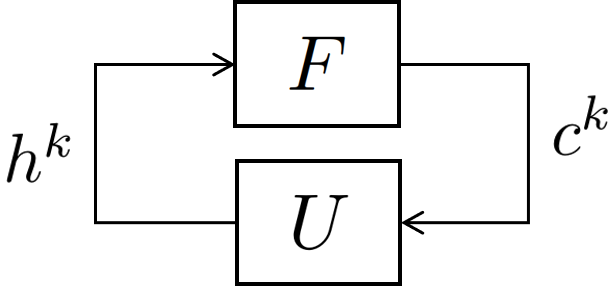
\includegraphics[width=0.4\linewidth]{figs/iteration.png}
    \caption{Generic iteration}
    \label{fig:iteartion}
\end{figure}

\subsection{Frank-Wolfe Algorithm (FW)}
FW 
\cite{fukushima1984modified} 
is a well-known method for solving convex optimization problems which is especially well suited for network problems. The algorithm was used in \cite{thai2016negative} to solve large-scale static traffic assignment problems. The update function of FW is,
\begin{equation}
h^{k+1} = h^k +\alpha\; (y^k - h^k)
\end{equation}
with $\alpha$ set such that $h^{k+1}$ minimized the cost function over the chord between 
$y^k$ and $h^k$.

% the following steps:
% \begin{enumerate}
% \item Compute $y^k$ with Eq. (\ref{eq:allornothing}).
% \item Calculate $d^k = $
% \item Calculate the step size $\alpha$ as the solution to the following line-search problem:
% \begin{equation}
% \begin{aligned}
% & \underset{\alpha}{\text{minimize}}
% & & \langle F(h^k + \alpha\; d^k), d^k \rangle \\
% & \text{subject to}
% & & \alpha \in [0,1]
% \end{aligned}
% \end{equation}
% \item $$.
% \end{enumerate}

% Terminate if Eq. (\ref{termination_criterion}) is met.

\subsection{Method of Successive Averages}
The Method of Successive Averages (MSA) is a heuristic that does not guarantee convergence to a solution, but has generally been found to work well \cite{nie2010solving}. The algorithm advances with,
\begin{equation}
h^{k+1} = (1-1/k)h^k + (1/k) y^k
\end{equation}

% \begin{enumerate}
% \item Compute $y^k$ with Eq. (\ref{eq:allornothing}).
% \item With step size $\alpha = 1/k$,  . 
% \end{enumerate}
% Terminate if Eq. (\ref{termination_criterion}) is met.

\subsection{Extra Projection Method}
The Extra Projection Method (EPM) is based on the Euclidean projection operator, defined as,
\begin{equation}
\Pi_\mathcal{H}(x) = \underset{h}{\text{argmin}}\{\lVert h-x\rVert_2 \; : \;h \in\mathcal{H} \}
\end{equation}
%where $\lVert\cdot\rVert$ is the Euclidean norm. 
The EPM guarantees convergence when $F$ is Lipschitz continuous and pseudo-monotone \cite{nie2010solving}. 
%Use $L$ to denote the Lipschitz constant of $F$. 
$\tau^k$ is a number that is smaller than the Lipschitz constant of $F$. The update function of EPM is,
\begin{equation}
h^{k+1} = \Pi_\mathcal{H}(h^k - \tau^k F(z^k))
\end{equation}
where $z^k = \Pi_\mathcal{H}(h^k - \tau^k c^k)$. If the Lipschitz constant of $F$ is unknown, then \cite{nie2010solving} proposes the following update equation for $\tau^k$:
\begin{equation}
\tau^{k+1} = \left\{
\begin{tabular}{ll}
$\sigma\;\tau^k$ & 
if $y^{k+1}-y^k < 0$ and $\frac{|y^{k+1}-y^k|}{|y^k|}> \mu$ \\
$\tau^k$ & otherwise
\end{tabular}
\right.
\end{equation}
%Here $y^{k+1}$ and $y^k$ are the all-or-nothing assignments corresponding to $h^k$ and $h^{k+1}$ respectively. 
$\mu$ and $\sigma$ are scalars between 0 and 1.


\section{Software}
\label{sec:software}
\begin{figure}[h]
    \centering
    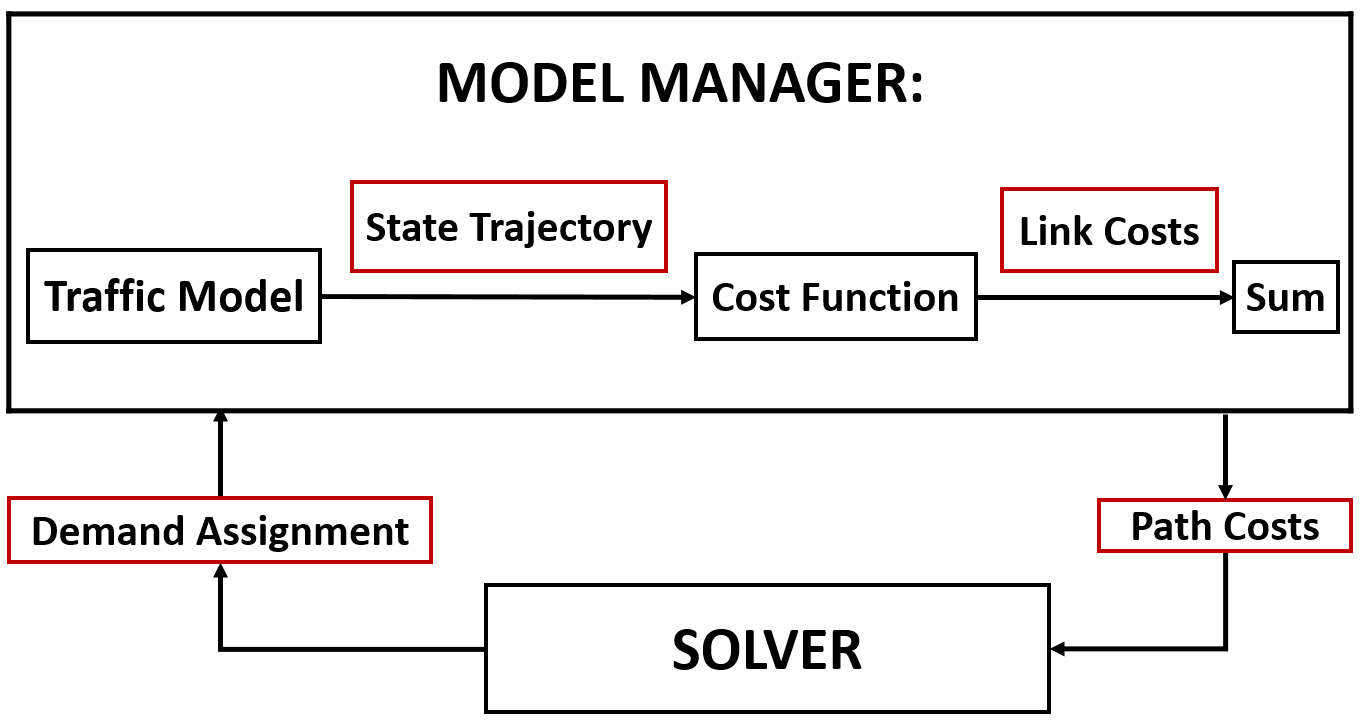
\includegraphics[width=0.7\linewidth]{figs/Software_Block_Diagram.PNG}
    %\caption{Software framework has a modular design, which allows to easily extend the framework.}
    \caption{Software design.}
    \label{fig:Block_Diagram}
\end{figure}

Using the VI formulation and the generic iteration shown in Figure \ref{fig:iteartion}, we designed a modular and extensible software framework to solve traffic assignment problems, including static and dynamic traffic problems. Figure~\ref{fig:Block_Diagram} show that the software framework has two main modules: the Model Manager and the Solver modules. The Demand Assignment and Path Costs components are wrappers for demand assignment $h$, and for path travel costs respectively $c$.

The Model Manager has three components that correspond to function $F$: the Traffic Model, Cost Function and Sum components. The software framework currently include three traffic models: ST, MN, and CTM, which all integrate in the framework via the Traffic Model component. These are implemented using the BeATS simulator \cite{beats}, which is an open-source implementation of the dynamic traffic models resported in this paper.  The State Trajectory module is a wrapper for link states (e.g: flow per link), and the Link Cost module is a wrapper for the travel cost per link (e.g experienced travel time on a link). The Model Manager's role is to translate an assignment $h$, specified as a sequence of demand per path by the Demand Assignment module, into the corresponding path costs, represented as a sequence of cost per path.

The Solver module serves as an interface to plug in solution algorithms for DTA. The Solver works in a loop (as described in Figure \ref{fig:iteartion}) in which it generates candidate demand assignments, and expects to be given the corresponding network path costs. This loop continues until an equilibrium demand assignment is reached. The Solver interface allows to incorporate different DTA solution algorithm. We included three solver algorithms: the MSA, the FW, and the EPM, which can be applied depending on the $F$ function properties. 

The advantage of our modular software framework is that it can be easily extended to address different traffic assignment problems by including new traffic models, cost functions, and solver algorithms. For example, the framework has a travel time based cost function. A user can add an energy or emission based cost function. For problems, such as simulation-based DTA problems, where the traffic model is tightly coupled with the cost function evaluation, a user can integrate implementation of the $F$ function without having to write the Traffic model, Cost Function and Sum modules. The complete documentation on software framework, with installations instructions can be found at \cite{ta_solver}.

\section{Experiments}
\label{sec:experiments}
In this section we demonstrate the methods described so far and implemented in the software using a simple scenario. The network, shown in Figure \ref{fig:config}, has six links numbered 0 through 5. Links 0 through 4 have flow capacities of 2,000 veh/hour, while link 5 has a capacity of 1,000 veh/hour. All links except for link 2 are 200 meters in length. Link 2 is 400 meters. The free-flow speed in all links is 70 km/hr, and hence the free-flow travel time for all links except link 2 is about 10 seconds, while for link 2 it is about 20 seconds. There are two origin/destination pairs: OD 1, going from source node 0 to sink node 5, and OD 2, going from source node 1 to sink node 5. There are two paths available to OD 1: path 1, consisting of links [0, 3, 4, 5], and path 2 consisting of links [0, 2, 4, 5]. OD 2 is confined to path 3 = [1, 3, 4, 5]. Path [1, 2, 4, 5] is not utilized.

This network was chosen because it is small enough that the results are intuitive, and yet it illustrates the essential differences between the models and travel time functions described in Section~\ref{sec:models}. Only OD pair 1 has a choice of route, and hence the assignment problem is only to decide how the demand for OD 1 should be split between paths 1 and path 2 during each time interval. The total demand for both ODs will be set to a value that exceeds the capacity of link 5, and hence we expect congestion to form and propagate upstream past link 4, and onto to links 2 and 3, regardless of the assignment. Because path 1 is shorter than path 2, OD 1 should choose path 1 until the accumulated congestion on link 3 causes its travel time to be as large or larger than that of link 2. Then the assignment should distribute traffic on paths 1 and 2 such that the travel times on links 2 and 3 are equalized. 

\begin{figure}[h]
    \centering
    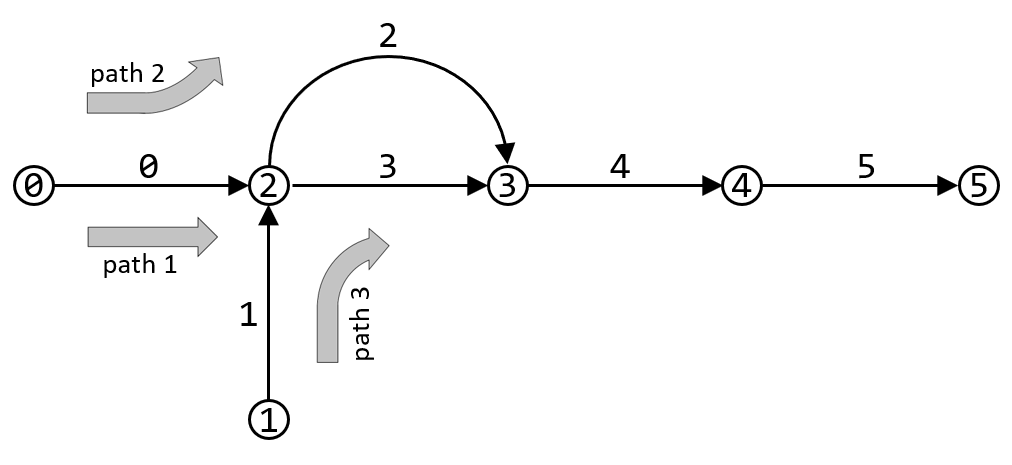
\includegraphics[width=\linewidth]{figs/config.png}
    \caption{Traffic network.}
    \label{fig:config}
\end{figure}

\subsection{Static assignment}
The static assignment problem with BPR cost function is the simplest case of traffic assignment. It can be posed as a convex optimization problem and solved efficiently with the Frank-Wolfe procedure. Figure~\ref{fig:static} shows solutions obtained with OD demands set to $d_0$=1300 veh/hr, $d_1$=300 veh/hr, and $\gamma$ ranging from 0 to 20. Equilibria with $h_1\neq 0$ and $h_2\neq 0$ are characterized by $\tau_2=\tau_3$. Using Eq.~\ref{eq:bpr}), feasibility ($h_1+h_2=d_0$ and $h_3=d_1$), and $\tau^0_2=2\;\tau^0_3$, this leads to,
\begin{equation}
\bar{f}^4 + \gamma\left(\;2(d_0-h_1)^4 - (d_1+h_1)^4 \;\right) = 0
\end{equation}
\todo[inline]{what is $\gamma$? Seems to not have been define, Juliette}
The root locus method \cite{rootlocus} can be applied here to track the trajectory of real solutions of this equation for $\gamma$'s ranging from zero to infinity.

% See Figure~\ref{fig:rlocus}. 
In the limit as $\gamma\rightarrow\infty$, the equilibrium value of $h_1$ decreases to 569.14 (the smallest real root of $2(d_0-h_1)^4 - (d_1+h_1)^4$), and $h_2=1300-h_1$ increases to 730.86. Thus, paradoxically, for $\gamma$ larger than a threshold, the number of vehicles that choose path 2 exceed those that choose path 1, even though path 2 is longer than path 1. This observation should be seen as a shortcoming of the BPR function as a model of travel time.

\begin{figure}[h]
    \centering
    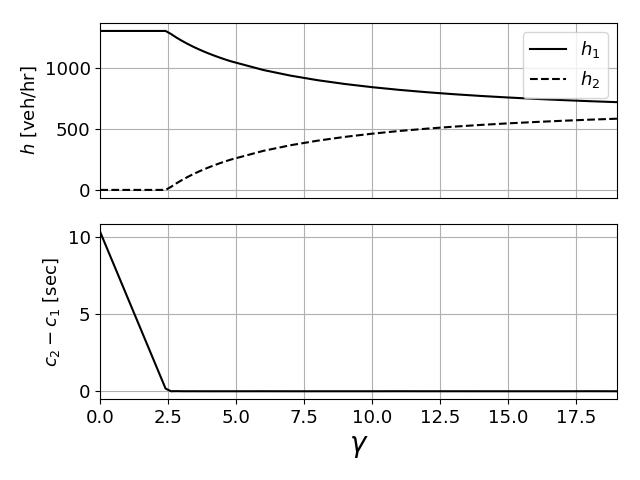
\includegraphics[width=0.8\linewidth]{figs/static.png}
    \caption{Static equilibria as a function of $\gamma$.}
    \label{fig:static}
\end{figure}

% \begin{figure}[h]
%     \centering
%     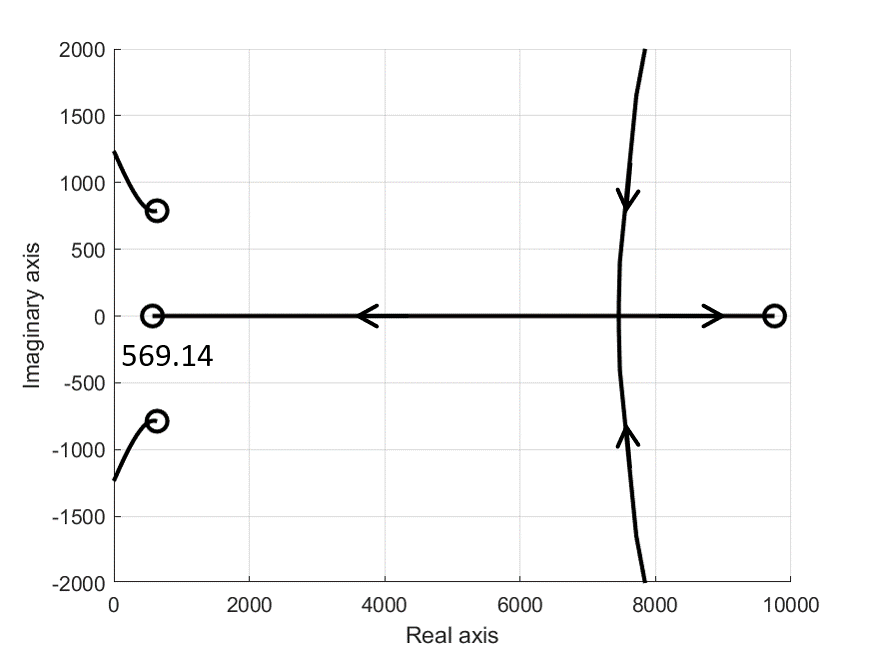
\includegraphics[width=0.8\linewidth]{figs/rlocus_mod.png}
%     \caption{Root locus.}
%     \label{fig:rlocus}
% \end{figure}

\subsection{Dynamic assignment}
Next we compute the dynamic equilibrium assignments under three different models: the MN model, the CTM model with instantaneous travel time, and the CTM with predictive travel time. The time period is 600 seconds. Demands are set to $d_0$=1300 and $d_1$=300 for time $\in[0,300]$ seconds, and $d_0$=$d_1$=0 thereafter. EPM was used to compute the solution, with an initial guess provided by MSA. The three solutions are shown in Figure~\ref{fig:ctm_vs_mn_hc}. The optimal assignment under the MN model places all of $d_0$ on path 1 for all times before 300 seconds, and so link 2 remains unused. This is because MN does not propagate congestion upstream, and so link 3 never slows down. This can be seen in Figure~\ref{fig:ctm_vs_mn_x}, where link 4 accumulates vehicles without bound up to 300 seconds. 
\begin{figure}[h]
    \centering
    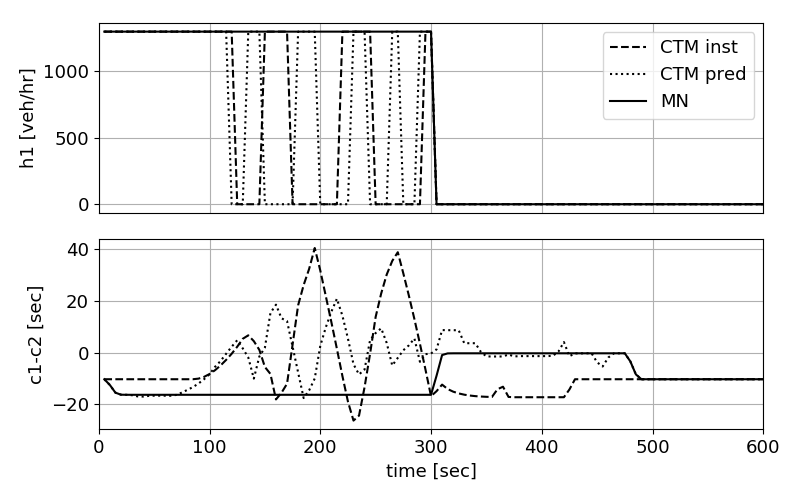
\includegraphics[width=\linewidth]{figs/ctm_vs_mn_hc.png}
    \caption{ctm vs mn hc}
    \label{fig:ctm_vs_mn_hc}
\end{figure}

\begin{figure}[h]
    \centering
    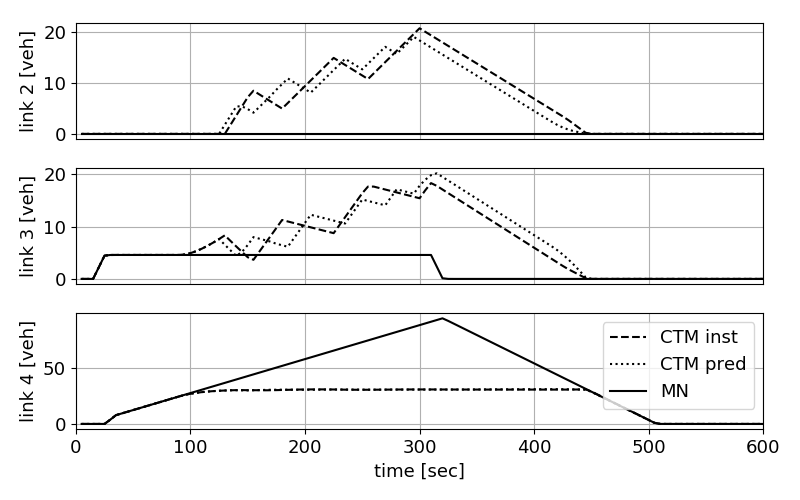
\includegraphics[width=\linewidth]{figs/ctm_vs_mn_x.png}
    \caption{ctm vs mn x}
    \label{fig:ctm_vs_mn_x}
\end{figure}
The two CTM solutions display behavior that is more realistic. In both cases, the entire demand is initially sent on path 1, since $c_2-c_1$ is positive, as can be seen in Figure~\ref{fig:ctm_vs_mn_hc}. The congestion on link 4 spills to link 3 after around 100 seconds, and at this point $c_2-c_1$ begins to decrease. Notice that the predictive version of travel time reacts before congestion reaches link 3. The travel times on paths 1 and 2 are equalized at around 116 seconds for CTM predictive, and 121 seconds for CTM instantaneous. At this point, the demand is shifted entirely to path 2. The effect of this change is delayed by the travel time on link 0. In the meantime, $c_1$ continues to increase, and hence $c_2-c_1$ becomes negative. After the pulse reaches links 2 and 3, the travel time on path 1 decreases rapidly, and travel time on path 2 increases. $c_2-c_1$ again becomes positive, and another oscillation begins. 

\begin{figure}[h]
    \centering
    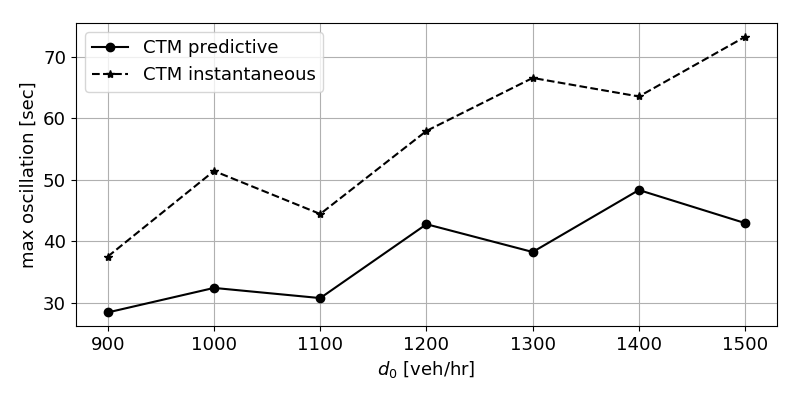
\includegraphics[width=0.8\linewidth]{figs/peaks.png}
    \caption{peaks }
    \label{fig:peaks}
\end{figure}

An immediate question is whether these oscillations are realistic. We do not attempt here to answer this question, but limit ourselves to a quantification of their size. Figure~\ref{fig:peaks} shows the maximum difference between consecutive peaks and valleys observed in the equilibrium assignment for a range of values for $d_0$ (from 900 vph to 1500 vph). Notice that the maximum oscillation with predictive travel time is uniformly smaller than that with instantaneous travel time. It is not clear to us at this point whether these oscillations are a property of the equilibrium solutions, a consequence of the discretization scheme, or related to the numerical solution methods. 

\begin{figure}[h]
    \centering
    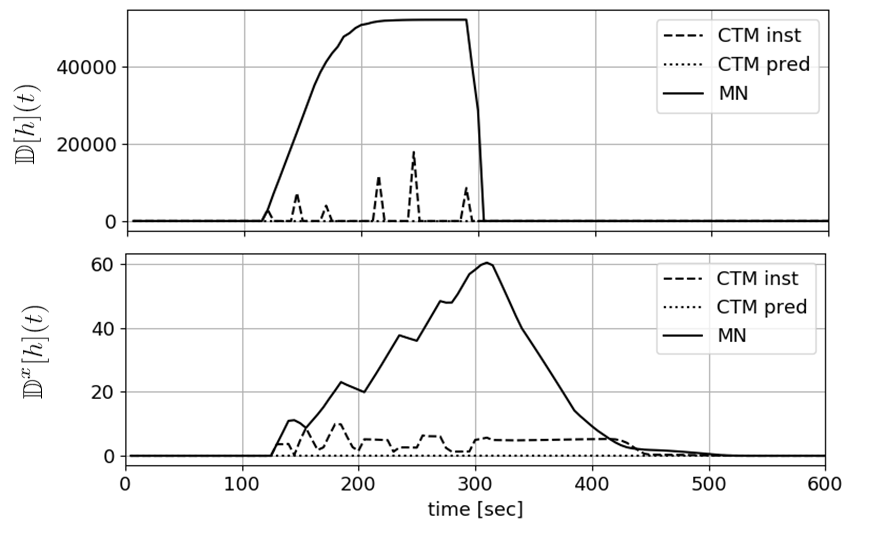
\includegraphics[width=\linewidth]{figs/DWardrop.png}
    \caption{DWardrop}
    \label{fig:dWardrop}
\end{figure}

% \begin{figure}[h]
%     \centering
%     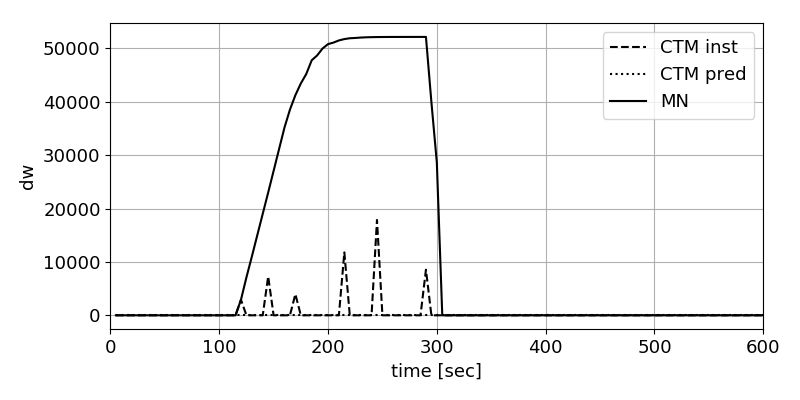
\includegraphics[width=\linewidth]{figs/dw.png}
%     \caption{dw}
%     \label{fig:dw}
% \end{figure}

Finally, we evaluate these three solutions in terms of their similarity to a Wardrop user equilibrium. To build a `distance to Wardrop' function, we express Wardrop's principle as a complementarity condition: $h^*$ is an equilibrium  if it is feasible and for all time $t$, all OD pairs $w$, and all paths $p\in\mathcal{P}_w$,
\begin{equation}
\label{eq:comp}
h_p(t)\left(c_p(t)-\pi_w(t)\right) = 0
\end{equation}
where $\pi_w(t)$ is the minimum travel time among paths in $\mathcal{P}_w$. The left hand side of Eq. (\ref{eq:comp}) is positive for all feasible assignments, and zero only for equilibrium assignments. Therefore the function,
\begin{equation}
\mathbb{D}[h](t) =\sum_w \sum_{p\in\mathcal{P}_w} h_p(t)\left(c_p(t)-\pi_w(t)\right)
\end{equation}
can serve as a rough measure of `distance to Wardrop', although it does not satisfy the triangle inequality nor the uniform scaling requirements of a norm. Computation $\mathbb{D}[h](t)$ requires a model to provide the travel times $c_p(t)$ corresponding to $h$. Here we use the CTM with predictive travel time, since it is the model that most closely matches our intuitions about the outcomes of the experiment. The results are shown in Figure~\ref{fig:dWardrop}. Clearly the equilibrium due to the MN model is farther from a Wardrop equilibrium than either of the CTM results. A shortcoming of $\mathbb{D}[h](t)$ is that it only penalizes incorrect assignments $h(t)$ at time $t$. The lingering effects of vehicles sent on non-minimum paths are lost. If, however, the problem has a unique equilibrium solution, then the distance to that state trajectory can also be used to measure `distance to Wardrop'.
\begin{equation}
\mathbb{D}^x[h](t) = \sum_{l} ||x^{*}(t)-x(t)||
\end{equation}
Here, $x^{*}(t)$ and $x(t)$ are, respectively, the equilibrium state trajectory and the state trajectory due to $h$. This quantity is depicted in the lower plot of Figure~\ref{fig:dWardrop}. Notice that the error persists beyond $t$=300.

\section{Conclusions}
\label{sec:conclusions}

\section*{Acknowledgment}


\bibliographystyle{abbrv}
\bibliography{citation.bib}


\end{document}
